\documentclass[hyperref, a4paper]{article}

\usepackage{geometry}
\usepackage{titling}
\usepackage{titlesec}
\usepackage{enumitem}
\usepackage{footnote}
\usepackage{enumerate}
\usepackage{amsmath, amssymb, amsthm}
\usepackage{mathtools}
\usepackage{bbm}
\usepackage{cite}
\usepackage{graphicx}
\usepackage{subfigure}
\usepackage{physics}
\usepackage{siunitx}
\usepackage[version=4]{mhchem}
\usepackage{tikz}
\usepackage{xcolor}
\usepackage{listings}
\usepackage{autobreak}
\usepackage[ruled, vlined, linesnumbered]{algorithm2e}
\usepackage{nameref,zref-xr}
\zxrsetup{toltxlabel}
\zexternaldocument*[optics-]{../optics/optics}[optics.pdf]
\usepackage[colorlinks,unicode, urlcolor=cyan]{hyperref} % , linkcolor=black, anchorcolor=black, citecolor=black, urlcolor=black, filecolor=black
\usepackage{prettyref}

\newcommand{\opticsdoc}{\href{../optics/optics}{the optics notes}}

% Page style
\geometry{left=3.18cm,right=3.18cm,top=2.54cm,bottom=2.54cm}
\titlespacing{\paragraph}{0pt}{1pt}{10pt}[20pt]
\setlength{\droptitle}{-5em}
\preauthor{\vspace{-10pt}\begin{center}}
\postauthor{\par\end{center}}

% More compact lists 
\setlist[itemize]{itemindent=17pt, leftmargin=1pt}

% Math operators
\DeclareMathOperator{\timeorder}{T}
\DeclareMathOperator{\diag}{diag}
\DeclareMathOperator{\legpoly}{P}
\DeclareMathOperator{\primevalue}{P}
\DeclareMathOperator{\sgn}{sgn}
\newcommand*{\ii}{\mathrm{i}}
\newcommand*{\ee}{\mathrm{e}}
\newcommand*{\const}{\mathrm{const}}
\newcommand*{\suchthat}{\quad \text{s.t.} \quad}
\newcommand*{\argmin}{\arg\min}
\newcommand*{\argmax}{\arg\max}
\newcommand*{\normalorder}[1]{: #1 :}
\newcommand*{\pair}[1]{\langle #1 \rangle}
\newcommand*{\fd}[1]{\mathcal{D} #1}
\DeclareMathOperator{\bigO}{\mathcal{O}}

\newcommand{\mathscr}{\mathcal}

% TikZ setting
\usetikzlibrary{arrows,shapes,positioning}
\usetikzlibrary{arrows.meta}
\usetikzlibrary{decorations.markings}
\tikzstyle arrowstyle=[scale=1]
\tikzstyle directed=[postaction={decorate,decoration={markings,
    mark=at position .5 with {\arrow[arrowstyle]{stealth}}}}]
\tikzstyle ray=[directed, thick]
\tikzstyle dot=[anchor=base,fill,circle,inner sep=1pt]

% Algorithm setting
% Julia-style code
\SetKwIF{If}{ElseIf}{Else}{if}{}{elseif}{else}{end}
\SetKwFor{For}{for}{}{end}
\SetKwFor{While}{while}{}{end}
\SetKwProg{Function}{function}{}{end}
\SetArgSty{textnormal}

\newcommand*{\concept}[1]{{\textbf{#1}}}

% Embedded codes
\lstset{basicstyle=\ttfamily,
  showstringspaces=false,
  commentstyle=\color{gray},
  keywordstyle=\color{blue}
}

\title{Quantum Optics, Homework 1}
\author{Jinyuan Wu}

\begin{document}

\maketitle

This document has been revised to include contents on the discussion session held on October 10, 2021.

\paragraph{}

\paragraph{Scully 1.1} The radiation field in an empty cubic cavity of side $L$ satisfies the wave equation
\begin{equation}
    \nabla^{2} \vb*{A}-\frac{1}{c^{2}} \frac{\partial^{2} \vb*{A}}{\partial t^{2}}=0
    \label{eq:scully-1-1-1}
\end{equation}
together with the Coulomb gauge condition $\nabla \cdot \vb*{A}=0$. Show that the solution that satisfies the boundary conditions has components
\begin{equation}
    \begin{aligned}
        &A_{x}(\vb*{r}, t)=A_{x}(t) \cos \left(k_{x} x\right) \sin \left(k_{y} y\right) \sin \left(k_{z} z\right), \\
        &A_{y}(\vb*{r}, t)=A_{y}(t) \sin \left(k_{x} x\right) \cos \left(k_{y} y\right) \sin \left(k_{z} z\right), \\
        &A_{z}(\vb*{r}, t)=A_{z}(t) \sin \left(k_{x} x\right) \sin \left(k_{y} y\right) \cos \left(k_{z} z\right),
        \end{aligned}
    \label{eq:scully-1-1-2}
\end{equation}
where $\vb*{A}(t)$ is independent of position and the wave vector $\vb*{k}$ has components given by Eq. (1.1.21). Hence show that the integers $n_{x}, n_{y}, n_{z}$ in Eq. (1.1.21) are restricted in that only one of them can be zero at a time.

\paragraph{Solution} The boundary condition concerning the vector potential is
\[
    \vb*{n} \times (\vb*{A}_1 - \vb*{A}_2) = 0, \quad \vb*{n} \cdot (\curl{\vb*{A}_1} - \curl{\vb*{A}_2}) = 0.
\]
Since under the Coulomb gage condition
\[
    \vb*{E} = - \pdv{\vb*{A}}{t}, \quad \vb*{B} = \curl{\vb*{A}}
\]
and both of them vanish outside the cavity, the vector potential is a spacial and temporal constant outside the cavity.
We are free to add a global constant to $\vb*{A}$, and the most convenient choice is to let $\vb*{A} = 0$ outside the cavity, so the boundary condition is just
\[
    \vb*{n} \times \vb*{A} = 0, \quad \vb*{n} \cdot (\curl{\vb*{A}}) = 0
\]
inside the cavity.

The first condition reads $A_x = A_y = 0$ on the $z=0$ plane and $z=L$ plane, $A_x = A_z = 0$ on the $y=0$ plane and the $y=L$ plane, and $A_y = A_z = 0$ on the $x=0$ plane and $x=L$ plane, which \emph{do not} mix the three components of $\vb*{A}$ together, so solving \eqref{eq:scully-1-1-1} with the boundary condition $\vb*{n} \times \vb*{A} = 0$ is just solving
\begin{equation}
    \laplacian A_i - \frac{1}{c^2} \pdv[2]{A_i}{t} = 0, \quad i = x, y, z
    \label{eq:scully-1-1-components-sep}
\end{equation}
separately for all the three components.
The problem for $A_x$ is 
\begin{equation}
    \left( \pdv[2]{x} + \pdv[2]{y} + \pdv[2]{z} \right) A_x - \frac{1}{c^2} \pdv[2]{A_x}{t} = 0, \quad A_x|_{y=0} = A_x|_{y=L} = A_x|_{z=0} = A_x|_{z=L} = 0.
    \label{eq:scully-1-1-x-problem}
\end{equation}
By separation of variables we seek a solution in the form of
\[
    A_x(\vb*{r}, t) = A_{x,xt}(x, t) A_{xy}(y) A_{xz}(z),
\]
and the equations for $A_{x, xt}, A_{xy}, A_{xz}$ are
\[
    \left( \pdv[2]{x} - k_y^2 - k_z^2 \right) A_{x, xt} - \frac{1}{c^2} \pdv[2]{A_{x, xt}}{t} = 0, \quad \pdv[2]{A_{xy}}{y} + k_y^2 = 0, \quad \pdv[2]{A_{xz}}{z} + k_z^2 = 0,
\]
respectively. Imposing boundary conditions to \eqref{eq:scully-1-1-x-problem} to $A_{xy}$ and $A_{xz}$ we obtain
\[
    A_{xy}(y) = \text{const} \times \sin(k_y y) , \quad A_{xz}(z) = \text{const} \times \sin(k_z z),
\]
where
\begin{equation}
    k_y = \frac{2\pi n_y}{L}, \quad k_z = \frac{2\pi n_z}{L}, \quad n_y, n_z \in \mathbb{Z},
    \label{eq:scully-1-1-ky-kz-conds}
\end{equation}
and we find $A_{x}$ has the form
\begin{equation}
    A_{x}(\vb*{r}, t) = A_{x, xt}(x, t) \sin(k_{xy} y) \sin(k_{xz} z), \quad k_{xy} = \frac{2\pi n_{xy}}{L}, k_{xz} = \frac{2\pi n_{xz}}{L}, \quad n_{xy}, n_{xz} \in \mathbb{Z}.
    \label{eq:scully-1-1-ax-form}
\end{equation}
Similarly we solve \eqref{eq:scully-1-1-components-sep} for $A_y$ and the result is
\begin{equation}
    A_{y}(\vb*{r}, t) = A_{y, yt}(y, t) \sin(k_{yx} x) \sin(k_{yz} z), \quad k_{yx} = \frac{2\pi n_{yx}}{L}, k_{yz} = \frac{2\pi n_{yz}}{L}, \quad n_{yx}, n_{yz} \in \mathbb{Z},
    \label{eq:scully-1-1-ay-form}
\end{equation}
and for $A_z$ the result is
\begin{equation}
    A_{z}(\vb*{r}, t) = A_{z, zt}(z, t) \sin(k_{zx} x) \sin(k_{zy} y), \quad k_{zx} = \frac{2\pi n_{zx}}{L}, k_{zy} = \frac{2\pi n_{zy}}{L}, \quad n_{zx}, n_{zy} \in \mathbb{Z},
    \label{eq:scully-1-1-az-form}
\end{equation}

Now the Coulomb gauge condition is just
\[
    \pdv{A_{x, xt}}{x} \sin(k_{xy} y) \sin(k_{xz} z) + \pdv{A_{y, yt}}{y} \sin(k_{yx} x) \sin(k_{yz} z) + \pdv{A_{z, zt}}{z} \sin(k_{zx} x) \sin(k_{zy} y) = 0.
\]
This equation holds only when
\[
    k_{xy} = k_{zy}, \quad k_{xz} = k_{yz}, \quad k_{yx} = k_{zx},
\]
and
\[
    \pdv{A_{x, xt}}{x} \propto \sin(k_{yx} x), \quad \pdv{A_{y, yt}}{y} \propto \sin(k_{xy} y) , \quad \pdv{A_{z, zt}}{z} \propto \sin(k_{yz} z).
\]
We therefore rename $k_{yx}$ as $k_x$, $k_{xz}$ as $k_z$, and $k_{xy}$ as $k_y$, and we have
\[
    A_{x, xt} \propto \cos(k_x x), \quad A_{y, yt} \propto \cos(k_y y), \quad A_{z, zt} \propto \cos(k_x z),
\]
so finally, we have 
\[
    A_x(\vb*{r}, t) = \text{some function of $t$} \times \cos \left(k_{x} x\right) \sin \left(k_{y} y\right) \sin \left(k_{z} z\right)
\]
and similar equations for $A_y$ and $A_z$,where $k_x, k_y, k_z$ all satisfy Eq.~(1.1.21), and thus we have proved \eqref{eq:scully-1-1-2}.

Now if $n_x = n_y = n_z$, then $\vb*{k} = 0$. Hence $\sin(k_i r_i), i = x, y, z$ are constantly zero, and \eqref{eq:scully-1-1-2} is an all-zero trivial solution.
If two of the integers $n_x, n_y, n_z$ are zero, say, $n_x = n_y = 0$, that still makes \eqref{eq:scully-1-1-2} an all-zero solution.
That explains why only one of them can be zero at a time.

\paragraph{Comment} A much more convenient way to do the job is just introducing a plane wave trial solution.
\eqref{eq:scully-1-1-2} does not have deep physical implication. It is just a demonstration of how separation of variables can be used even in quantum optics.

\paragraph{}

\paragraph{Scully 1.2} If $A$ and $B$ are two noncommuting operators that satisfy the conditions
\begin{equation}
    [[A, B], A]=[[A, B], B]=0,
    \label{eq:scully-1-2-1}
\end{equation}
then show that
\begin{equation}
    \begin{aligned}
        \ee^{A+B} &= \ee^{-\frac{1}{2}[A, B]} \ee^{A} \ee^{B} \\
        &= \ee^{+\frac{1}{2}[A, B]} \ee^{B} \ee^{A}.
    \end{aligned}
    \label{eq:scully-1-2-2}    
\end{equation}
This is a special case of the so-called Baker-Hausdorff theorem of group theory.

\paragraph{Solution} To show \eqref{eq:scully-1-2-2} it is sufficient to prove 
\begin{equation}
    \ee^{A} \ee^{B} = \ee^{A + B + \frac{1}{2} \comm*{A}{B}},
    \label{eq:scully-1-2-2-origin}
\end{equation}
as $\comm*{A}{B}$ commutes with both $A$ and $B$ and therefore commute with $\ee^A$ and $e^B$.
To prove \eqref{eq:scully-1-2-2-origin}, we define an operator function $G(x)$ by 
\begin{equation}
    \ee^{x A} \ee^{x B} = \ee^{G(x)}.
    \label{eq:scully-1-2-temp-5}
\end{equation}
When $x=0$, $\ee^{G(x)} = 1$, so $G(x) = 0$, and we have Taylor series of $G(x)$ at $x=0$:
\[
    G(x) = x G_1 + x^2 G_2 + \cdots.
\]
Now consider the trivial equation
\begin{equation}
    \ee^{- xB} \ee^{- xA} \dv{x} \left( \ee^{x A} \ee^{x B} \right) = \ee^{-G(x)} \dv{x} \ee^{G(x)},
    \label{eq:scully-1-2-temp-1}
\end{equation}
where LHS is 
\begin{equation}
    \begin{aligned}
        \ee^{- xB} \ee^{- xA} \dv{x} \left( \ee^{x A} \ee^{x B} \right) &=  \ee^{- xB} \ee^{- xA} (A \ee^{x A} \ee^{x B} + \ee^{x A} B \ee^{x B}) \\
        &= \ee^{-xB} A \ee^{xB} + B.
    \end{aligned}
    \label{eq:scully-1-2-temp-2}
\end{equation}

Now we need an important equation:
\begin{equation}
    \ee^{G} A \ee^{-G} = A + \comm*{G}{A} + \frac{1}{2!} [G, [G, A]] + \cdots + \frac{1}{n!} \underbrace{[G,[G,[G, \ldots[G, A]]] \ldots]}_{n \text { times }} + \cdots. 
    \label{eq:scully-1-2-temp-4}
\end{equation}
We use the proof given by \cite{711309}. By definition we have
\[
    \begin{aligned}
        \ee^{G} A \ee^{-G} &= \sum_{m=0}^\infty \frac{1}{m!} G^m A \sum_{n=0}^\infty \frac{1}{n!} (-G)^n \\
        &= \sum_{m=0}^\infty \sum_{n=0}^\infty \frac{1}{m! n!} (-1)^n G^m A G^n \\
        &= \sum_{s=0}^\infty \sum_{n=0}^\infty \frac{1}{(s-n)! n!} (-1)^n G^{s-n} A G^n \\
        &= \sum_{s=0}^\infty \frac{1}{s!} \sum_{n=0}^\infty \binom{s}{n} (-1)^n G^{s-n} A G^n \\
        &= A + [G, A] + \cdots + \frac{1}{s!} \sum_{n=0}^s \binom{s}{n} (-1)^n G^{s-n} A G^n + \cdots,
    \end{aligned}
\]
so the problem is whether 
\begin{equation}
    \sum_{k=0}^n \binom{n}{k} (-1)^k G^{n-k} A G^k =  \underbrace{[G,[G,[G, \ldots[G, A]]] \ldots]}_{n \text { times }}.
    \label{eq:scully-1-2-temp-3}
\end{equation}
\eqref{eq:scully-1-2-temp-3} can be shown recursively. The cases of $n=1, 2$ are trivial. Suppose \eqref{eq:scully-1-2-temp-3} for an arbitrary $n$, then 
\[
    \begin{aligned}
        &\quad \underbrace{[G,[G,[G, \ldots[G, A]]] \ldots]}_{n+1 \text { times }} \\
        &= \sum_{k=0}^n \binom{n}{k} (-1)^k G^{n-k} \comm*{G}{A} G^k \\
        &= \sum_{k=0}^n \binom{n}{k} (-1)^k G^{n-k + 1} A G^k - G^{n-k} A G^{k+1}) \\
        &= \sum_{k=1}^n \binom{n}{k} (-1)^k (G^{n-k + 1} A G^k + G^{n+1} A - \sum_{k=1}^n \binom{n}{k-1} (-1)^{k-1} G^{n - k+1} A G^k - (-1)^n A G^{n+1} \\
        &= G^{n+1} A - (-1)^n A G^{n+1} + \sum_{k=1}^n \left( \binom{n}{k} + \binom{n}{k-1} \right) (-1)^k G^{n-k + 1} A G^k \\
        &=  G^{n+1} A - (-1)^n A G^{n+1} + \sum_{k=1}^n \binom{n+1}{k} (-1)^k G^{n-k + 1} A G^k \\
        &= \sum_{k=0}^{n+1} \binom{n+1}{k} (-1)^k G^{n-k + 1} A G^k ,
    \end{aligned}
\]
which is just \eqref{eq:scully-1-2-temp-3} with $n$ replaced by $n+1$.
So \eqref{eq:scully-1-2-temp-3} has been proven.

Now due to \eqref{eq:scully-1-2-temp-4}, the RHS of \eqref{eq:scully-1-2-temp-2} is 
\[
    B + \ee^{-xB} A \ee^{xB} = B + A + \comm*{-xB}{A}.
\]
All higher order terms contain $\comm*{B}{\comm*{B}{A}}$ and therefore vanish.
The RHS of \eqref{eq:scully-1-2-temp-1} can be evaluated as
\[
    \begin{aligned}
        \ee^{-G(x)} \dv{x} \ee^{G(x)} &= \ee^{-G(x)} \sum_{m=0}^\infty \sum_{n=0}^\infty \frac{1}{(m+n+1)!} G^m G' G^n ,
    \end{aligned}
\]
and by the integral formula 
\[
    \int_{0}^{1} \dd y(1-y)^{n} y^{m}=\frac{n ! m !}{(n+m+1) !}
\]
we have 
\[
    \begin{aligned}
        \ee^{-G(x)} \dv{x} \ee^{G(x)} &= \ee^{-G(x)} \sum_{m=0}^\infty \sum_{n=0}^\infty \frac{1}{m! n!} \int_{0}^{1} \dd{y} (1-y)^{n} y^{m} G^m G' G^n \\
        &= \ee^{-G(x)} \int_{0}^{1} \dd{y} \ee^{(1-y) G} G' \ee^{yG} \\
        &= \int_{0}^{1} \dd{y} \ee^{-y G} G' \ee^{yG} ,
    \end{aligned}
\]
and now it can be evaluated using \eqref{eq:scully-1-2-temp-4} as
\[
    \begin{aligned}
        \ee^{-G(x)} \dv{x} \ee^{G(x)} &= \int_0^1 \dd{y} \left( G' + y \comm*{G'}{G} + \frac{y^2}{2} \comm*{\comm*{G'}{G}}{G} + \bigO(y^3) \right) \\
        &= G' + \frac{1}{2} \comm*{G'}{G}  + \frac{1}{3!} \comm*{\comm*{G'}{G}}{G} + \cdots.
    \end{aligned}
\]
As $G(x)$ can be expanded into
\[
    G'(x) = G_1 + 2x G_2 + \cdots,
\]
We have
\[
    \ee^{-G(x)} \dv{x} \ee^{G(x)} = G_1 + 2 x G_2 + \frac{1}{2} x^2 \comm*{G_2}{G_1} + \cdots.
\]
So finally, by rewriting its LHS and RHS, from \eqref{eq:scully-1-2-temp-1} we find that 
\[
    B + A + x [A, B] = G_1 + 2 x G_2 + \bigO(x^2),
\]
and thus
\[
    G_1 = A + B, \quad G_2 = \frac{1}{2} [A, B], \quad G_{n} = 0 \text{ for $n > 2$}.
\]
So 
\[
    G(x) = A + B + \frac{1}{2} \comm*{A}{B},
\]
and by taking $x=1$ in \eqref{eq:scully-1-2-temp-5} we complete the proof of \eqref{eq:scully-1-2-2-origin}, therefore have proved \eqref{eq:scully-1-2-2}.

\paragraph{Comment} Note that when \eqref{eq:scully-1-2-1} holds, we have 
\begin{equation}
    \ee^{2(A+B)} = \ee^{A} \ee^{B} \ee^{- \frac{1}{2} \comm*{A}{B}} \ee^{\frac{1}{2} \comm*{A}{B}} \ee^{B} \ee^{A} = \ee^{A} \ee^{2B} \ee^{A},
\end{equation}
or in other words
\begin{equation}
    \ee^{A+B} = \ee^{A/2} \ee^{B} \ee^{A/2} = \ee^{B/2} \ee^{A} \ee^{B/2}.
\end{equation}
This decomposition can be used to increase the accuracy of Trotter decomposition.
For example if the commuter of the kinetic energy and the potential energy of a particle almost commutes with themselves, then 
\begin{equation}
    \ee^{\ii \Delta t (K+V)} = \ee^{\ii \Delta t K / 2} \ee^{\ii \Delta t V} \ee^{\ii \Delta t K / 2}.
\end{equation}

\paragraph{}

\paragraph{Scully 1.4} If $f\left(a, a^{\dagger}\right)$ is a function which can be expanded in a power series of $a$ and $a^{\dagger}$, then show that
(a) $\left[a, f\left(a, a^{\dagger}\right)\right]=\frac{\partial f}{\partial a^{\dagger}}$,
(b) $\left[a^{\dagger}, f\left(a, a^{\dagger}\right)\right]=-\frac{\partial f}{\partial a}$,
(c) $\ee^{-\alpha a^{\dagger} a} f\left(a, a^{\dagger}\right) \ee^{\alpha a^{\dagger} a}=f\left(a \ee^{\alpha}, a^{\dagger} \ee^{-\alpha}\right)$
where $\alpha$ is a parameter.

\paragraph{Solution} Suppose
\begin{equation}
    f(a, a^\dagger) = \sum_{m, n \geq 0} f_{mn} a^m (a^\dagger)^n.
\end{equation}
We do not include terms that start with $a^\dagger$, because by $\comm*{a}{a^\dagger} = 1$ we can move all $a$ operators to the left.
We can also move all $a$ operators to the right, and write down a similar expansion
\begin{equation}
    f(a, a^\dagger) = \sum_{m, n \geq 0} g_{mn} (a^\dagger)^m a^n.
    \label{eq:normal-ordered-general-form}
\end{equation}
\begin{itemize}
\item[(a)] We have \[
    \begin{aligned}
        \comm*{a}{f(a, a^\dagger)} &= \sum_{m, n \geq 0} f_{mn} a^m \comm*{a}{(a^\dagger)^m} \\
        &= \sum_{m, n \geq 0} f_{mn} a^m \left( [a, a^\dagger] (a^\dagger)^{m-1} + a^\dagger [a, (a^\dagger)^{m-1}] \right) \\
        &= \sum_{m, n \geq 0} f_{mn} a^m \left( (a^\dagger)^{m-1} + a^\dagger [a, (a^\dagger)^{m-1}] \right) \\
        &= \sum_{m, n \geq 0} f_{mn} a^m \left( (a^\dagger)^{m-1} + a^\dagger \left( a^\dagger [a, (a^\dagger)^{m-2}] + \comm*{a}{a^\dagger} (a^\dagger)^{m-2} \right) \right) \\
        &= \sum_{m, n \geq 0} f_{mn} a^m \left( (a^\dagger)^{m-1} + a^\dagger \left( a^\dagger [a, (a^\dagger)^{m-2}] + (a^\dagger)^{m-2} \right) \right) \\
        &= \sum_{m, n \geq 0} f_{mn} a^m \left( 2 (a^\dagger)^{m-1} + (a^\dagger)^2 \comm*{a}{(a^\dagger)^{m-2}} \right) \\
        & = \cdots.
    \end{aligned}
\]
As the expansion of $\comm*{a}{(a^\dagger)^{m}}$ goes, we get a sequence of equations in the form of 
\[
    \begin{aligned}
        [a, f(a, a^\dagger)] &= \sum_{m, n \geq 0} f_{mn} a^m \left( (a^\dagger)^{m-1} + a^\dagger [a, (a^\dagger)^{m-1}] \right) \\
        &= \sum_{m, n \geq 0} f_{mn} a^m \left( 2(a^\dagger)^{m-1} + a^\dagger [a, (a^\dagger)^{m-2}] \right) \\
        &= \cdots,
    \end{aligned}
\]
and the sequence stops at 
\[
    \sum_{m, n \geq 0} f_{mn} a^m \left( m (a^\dagger)^{m-1} + a^\dagger \comm*{a}{(a^\dagger)^{m-m}} \right),
\] 
so we have 
\[
    \comm*{a}{f(a, a^\dagger)} = \sum_{m, n \geq 0} f_{mn} a^m m (a^\dagger)^{m-1} ,
\] 
and since 
\[
    \pdv{f}{a^\dagger} = \sum_{m, n \geq 0} f_{mn} a^m \pdv{(a^\dagger)^m}{a^\dagger},
\]
we arrive at the conclusion that
\begin{equation}
    \comm*{a}{f(a, a^\dagger)} = \pdv{f}{a^\dagger}.
    \label{eq:scully-1-4-result-1}
\end{equation}
\item[(b)] The logic is similar to (a) but this time the expansion is
\[
    \begin{aligned}
        \comm*{a^\dagger}{f(a, a^\dagger)} &= \sum_{m, n \geq 0} \comm*{a^\dagger}{a^m} (a^\dagger)^n \\
        &= \sum_{m, n \geq 0} \left( \comm*{a^\dagger}{a} a^{m-1} + a \comm*{a^\dagger}{a^{m-1}} \right) \\
        &= \sum_{m, n \geq 0} \left( - a^{m-1} + a \comm*{a^\dagger}{a^{m-1}} \right) \\
        &= \sum_{m, n \geq 0} \left( - a^{m-1} + a \left( a \comm*{a^\dagger}{a^{m-2}} \right) + \comm*{a^\dagger}{a} a^{m-2} \right) \\
        &= \sum_{m, n \geq 0} \left( - a^{m-1} + a \left( \left( a \comm*{a^\dagger}{a^{m-2}} \right) - a^{m-2} \right) \right) \\
        &= \sum_{m, n \geq 0} \left( - 2 a^{m-1} + a^2 \comm*{a^\dagger}{a^{m-2}} \right) \\
        &= \cdots,
    \end{aligned}
\]
or to be concise, 
\[
    \begin{aligned}
        \comm*{a^\dagger}{f(a, a^\dagger)} &= \sum_{m, n \geq 0} \left( - a^{m-1} + a \comm*{a^\dagger}{a^{m-1}} \right) \\
        &= \sum_{m, n \geq 0} \left( - 2 a^{m-1} + a^2 \comm*{a^\dagger}{a^{m-2}} \right) \\
        &= \cdots,
    \end{aligned}
\]
and this time the sequence stops at
\[
    \comm*{a^\dagger}{f(a, a^\dagger)} = \sum_{m, n \geq 0} \left( - m a^{m-1} + a^2 \comm*{a^\dagger}{a^{m-m}} \right),
\]
and since 
\[
    - m a^{m-1} = - \pdv{a^m}{a}
\]
we have
\begin{equation}
    \comm*{a^\dagger}{f(a, a^\dagger)} = - \pdv{f}{a}.
    \label{eq:scully-1-4-result-2}
\end{equation}
\item[(c)] We need to use results proved in Problem 1.5. By \eqref{eq:scully-1-5-1}, we have
\begin{equation}
    a \ee^{- \alpha a^\dagger a} = \ee^{- \alpha} \ee^{- \alpha a^\dagger a} a = (\ee^{-\alpha} a) \ee^{- \alpha a^\dagger a}, 
    \label{eq:scully-1-5-lemma-1}
\end{equation}
and by taking its conjugate transpose we have
\[
    a^\dagger \ee^{- \alpha^* a^\dagger a} \ee^{- \alpha^*} = \ee^{- \alpha^* a^\dagger a} a^\dagger,
\]
and since $\alpha$ is an arbitrary parameter we can redefine it and get
\begin{equation}
    a^\dagger \ee^{- \alpha a^\dagger a} \ee^{- \alpha} = \ee^{- \alpha a^\dagger a} a^\dagger = (a^\dagger \ee^{-\alpha}) \ee^{- \alpha a^\dagger a}.
    \label{eq:scully-1-5-lemma-2}
\end{equation}
Substituting \eqref{eq:normal-ordered-general-form} into $\ee^{-\alpha a^\dagger a} f(a, a^\dagger) \ee^{\alpha a^\dagger a}$, and applying \eqref{eq:scully-1-5-lemma-1} and \eqref{eq:scully-1-5-lemma-2} iteratively, we have
\[
    \begin{aligned}
        \ee^{-\alpha a^\dagger a} f(a, a^\dagger) \ee^{\alpha a^\dagger a} &= \sum_{n, m \geq 0} g_{mn} \ee^{-\alpha a^\dagger a} (a^\dagger)^m a^n \ee^{\alpha a^\dagger a} \\
        &= \sum_{n, m \geq 0} g_{mn} (\ee^{-\alpha} a^\dagger) \ee^{-\alpha a^\dagger a} (a^\dagger)^{m-1} a^{n-1} \ee^{\alpha a^\dagger a} (a \ee^{\alpha}) \\
        &= \sum_{n, m \geq 0} g_{mn} (\ee^{-\alpha} a^\dagger) (\ee^{-\alpha} a^\dagger) \ee^{-\alpha a^\dagger a} (a^\dagger)^{m-2} a^{n-2} \ee^{\alpha a^\dagger a} (a \ee^{\alpha}) (a \ee^{\alpha}) \\
        &= \cdots \\
        &= \sum_{m, n \geq 0} g_{mn} (\ee^{-\alpha} a^\dagger)^m \ee^{-\alpha a^\dagger a} \ee^{\alpha a^\dagger a} (\ee^{\alpha} a)^n \\
        &= \sum_{m, n \geq 0} g_{mn} (\ee^{-\alpha} a^\dagger)^m (\ee^{\alpha} a)^n \\
        &= f(a \ee^{\alpha}, a^\dagger \ee^{-\alpha}),
    \end{aligned}
\]
which finishes the proof.
\end{itemize}

\paragraph{Comment} Scully 1.4(c) actually gives the explicit time evolution of the creation operator and the annihilation operator.
Let 
\[
    \alpha = - \ii \omega t,
\]
then we have 
\[
    \ee^{\ii \omega a^\dagger a t} f(a, a^\dagger) \ee^{- \ii \omega a^\dagger a t} = f(\ee^{- \ii \omega t} a, \ee^{\ii \omega t} a^\dagger),
\]
which means
\begin{equation}
    \ee^{\ii H t / \hbar} f(a, a^\dagger) \ee^{- \ii H t / \hbar} = f(\ee^{- \ii \omega t} a, \ee^{\ii \omega t} a^\dagger).
\end{equation}
We see the equation implies that $a$ evolves as 
\[
    a(t) = a(0) \ee^{- \ii \omega t},
\]
which is true because 
\[
    \ii \hbar \dot{a} = \comm*{a}{H} = \hbar \omega a.
\]

\paragraph{}

\paragraph{Scully 1.5} Show that
\begin{equation}
    \begin{gathered}
        {\left[a, \ee^{-\alpha a^{\dagger} a}\right]=\left(\ee^{-\alpha}-1\right) \ee^{-\alpha a^{\dagger} a} a}, \\
        {\left[a^{\dagger}, \ee^{-\alpha a^{\dagger} a}\right]=\left(\ee^{\alpha}-1\right) \ee^{-\alpha a^{\dagger} a} a^{\dagger}},
        \end{gathered}
    \label{eq:scully-1-5-1}
\end{equation}
where $\alpha$ is a parameter.

\paragraph{Solution} The most convenient way is not to invoke \eqref{eq:scully-1-4-result-1} and \eqref{eq:scully-1-4-result-2}, but to check the matrix elements under the $\{\ket*{n}\}$ basis.
We have
\[
    \begin{aligned}
        \comm{a}{\ee^{-\alpha a^\dagger a}} \ket*{n} &= a \ee^{-\alpha a^\dagger a} \ket*{n} - \ee^{-\alpha a^\dagger a} a \ket*{n} \\
        &= a \ee^{- \alpha n} \ket*{n} - \ee^{- \alpha a^\dagger a} \sqrt{n} \ket*{n-1} \\
        &= \ee^{- \alpha n} \sqrt{n} \ket*{n-1} - \ee^{- \alpha (n-1)} \sqrt{n} \ket*{n-1} \\
        &= \left( \ee^{-\alpha} - 1 \right) \ee^{- \alpha (n-1)} \sqrt{n} \ket*{n-1} \\
        &= \left( \ee^{-\alpha} - 1 \right) \ee^{- \alpha a^\dagger a} \sqrt{n} \ket*{n-1} \\
        &= \left( \ee^{-\alpha} - 1 \right) \ee^{- \alpha a^\dagger a} a \ket*{n},
    \end{aligned}
\]
for all $n = 0, 1, \ldots$, and thus 
\begin{equation}
    \comm{a}{\ee^{-\alpha a^\dagger a}} = \left( \ee^{-\alpha} - 1 \right) \ee^{- \alpha a^\dagger a} a.
\end{equation}

The same procedure applies for the second equation. We have
\[
    \begin{aligned}
        \left[a^{\dagger}, \ee^{-\alpha a^{\dagger} a}\right] \ket*{n} &= a^\dagger \ee^{-\alpha a^{\dagger} a} \ket*{n} - \ee^{-\alpha a^{\dagger} a} a^\dagger \ket*{n} \\
        &= a^\dagger \ee^{-\alpha n} \ket*{n} - \ee^{-\alpha a^{\dagger} a} \sqrt{n+1} \ket*{n+1} \\
        &=  \ee^{-\alpha n} \sqrt{n+1} \ket*{n+1} - \ee^{-\alpha (n+1)} \sqrt{n+1} \ket*{n+1} \\
        &= \left( \ee^{\alpha} -1 \right) \ee^{-\alpha(n+1)} \sqrt{n+1} \ket*{n+1} \\
        &= \left( \ee^{\alpha} -1 \right) \ee^{-\alpha a^\dagger a} \sqrt{n+1} \ket*{n+1} \\
        &= \left( \ee^{\alpha} -1 \right) \ee^{-\alpha a^\dagger a} a^\dagger \ket*{n}, 
    \end{aligned}
\]
for all $n = 0, 1, \ldots$, and thus
\begin{equation}
    {\left[a^{\dagger}, \ee^{-\alpha a^{\dagger} a}\right]=\left(\ee^{\alpha}-1\right) \ee^{-\alpha a^{\dagger} a} a^{\dagger}}.
\end{equation}

\paragraph{}

\paragraph{Scully 1.6} Show that the free-field Hamiltonian
\begin{equation}
    \mathscr{H}=\hbar v\left(a^{\dagger} a+\frac{1}{2}\right)
    \label{eq:scully-1-6-free-field-ham}
\end{equation}
can be written in terms of the number states as
\[
\mathscr{H}=\sum_{n} E_{n}|n\rangle\langle n|,
\]
and hence
\begin{equation}
    \ee^{\ii \mathscr{H} t / \hbar}=\sum_{n} \ee^{\ii E_{n} t / \hbar}|n\rangle\langle n|.
    \label{eq:scully-1-6-3}
\end{equation}

\paragraph{Solution} An $n$-photon state
\begin{equation}
    \ket*{n} = \frac{1}{\sqrt{n!}} (a^\dagger)^n \ket*{0}
    \label{eq:scully-1-6-n-photon}
\end{equation}
is an eigenstate of \eqref{eq:scully-1-6-free-field-ham}, since by applying \eqref{eq:scully-1-6-free-field-ham} on \eqref{eq:scully-1-6-n-photon} we have
\[
    \begin{aligned}
        \mathcal{H} \ket*{n} &= \hbar \nu a^\dagger a \ket*{n} + \frac{1}{2} \hbar \nu \ket*{n} \\
        &= \hbar \nu a^\dagger \sqrt{n} \ket*{n-1} + \frac{1}{2} \hbar \nu \ket*{n} \\
        &= \hbar \nu \sqrt{n} \sqrt{n-1+1} \ket*{n-1+1} + \frac{1}{2} \hbar \nu \ket*{n} \\
        &= \hbar \nu \left( n + \frac{1}{2} \right) \ket*{n} \\
        &= E_n \ket*{n},
    \end{aligned}
\]
so $\ket*{n}$ is an eigenstate of $\mathcal{H}$ with energy $E_n$.
Since $\ket*{n}$s are orthogonal to each other and are uniform, we have
\begin{equation}
    \mathcal{H} = \sum_n E_n \dyad*{n}.
\end{equation}
Since $\mathcal{H}$ is diagonal under the $\{\ket*{n}\}$ basis, so is $\ee^{\ii \mathcal{H} t / \hbar}$ and hence we have \eqref{eq:scully-1-6-3}.

\paragraph{}

\paragraph{Scully 2.1} Show that
\begin{equation}
    a^\dagger \dyad*{\alpha} = \left( \alpha^{*}+\frac{\partial}{\partial \alpha} \right) \dyad*{\alpha},
    \label{eq:scully-2-1-1}
\end{equation}
and
\begin{equation}
    \dyad*{\alpha} a = \left(\alpha+\frac{\partial}{\partial \alpha^{*}}\right) \dyad*{\alpha}.
    \label{eq:scully-2-1-2}
\end{equation}

\paragraph{Solution} By definition
\[
    \dyad{\alpha} = \ee^{- \abs*{\alpha}^2} \sum_{n=0}^\infty \sum_{m=0}^\infty \frac{\alpha^n (\alpha^*)^m}{\sqrt{m! n!}} \dyad{n}{m},
\]
so 
\[
    \begin{aligned}
        a^\dagger \dyad{\alpha} &= \ee^{- \abs*{\alpha}^2} \sum_{n=0}^\infty \sum_{m=0}^\infty \frac{\alpha^n (\alpha^*)^m}{\sqrt{m! n!}} a^\dagger \dyad{n}{m} \\
        &= \ee^{- \abs*{\alpha}^2} \sum_{n=0}^\infty \sum_{m=0}^\infty \frac{\alpha^n (\alpha^*)^m}{\sqrt{m! n!}} \sqrt{n+1} \dyad{n+1}{m} \\
        &= \ee^{- \abs*{\alpha}^2} \sum_{n=0}^\infty \sum_{m=0}^\infty \frac{\alpha^n (\alpha^*)^m}{\sqrt{m! (n+1)!}} (n+1) \dyad{n+1}{m} \\
        &= \ee^{- \abs*{\alpha}^2 } \sum_{n=0}^\infty \frac{1}{\sqrt{(n+1)!}} \pdv{\alpha} \alpha^{n+1} \ket*{n+1} \sum_{m=0}^\infty \frac{ (\alpha^*)^m}{\sqrt{m!}} \bra{m} \\
        &= \ee^{- \abs*{\alpha}^2 } \sum_{n=1}^\infty \frac{1}{\sqrt{n!}} \left( \pdv{\alpha} \alpha^{n} \right) \ket*{n} \sum_{m=0}^\infty \frac{ (\alpha^*)^m}{\sqrt{m!}} \bra{m} .
    \end{aligned}
\]
Note that the factors after $\sum_m$ do not include $\alpha^*$, so they can be regarded as constants.
We have
\[
    \begin{aligned}
        \ee^{- \abs*{\alpha}^2 } \sum_{n=1}^\infty \frac{1}{\sqrt{n!}} \pdv{\alpha} \alpha^{n} \ket*{n} &= \ee^{- \abs*{\alpha}^2 } \pdv{\alpha} \sum_{n=0}^\infty \frac{1}{\sqrt{n!}} \alpha^{n} \ket*{n} \\
        &= \pdv{\alpha} \left( \ee^{- \abs*{\alpha}^2 } \sum_{n=0}^\infty \frac{1}{\sqrt{n!}} \alpha^{n} \ket*{n} \right) - \left(\pdv{\ee^{-\abs*{\alpha}^2 }}{\alpha}\right) \sum_{n=1}^\infty \frac{1}{\sqrt{n!}} \alpha^{n} \ket*{n} \\
        &= \pdv{\alpha} \left( \ee^{- \abs*{\alpha}^2 } \sum_{n=0}^\infty \frac{1}{\sqrt{n!}} \alpha^{n} \ket*{n} \right) - (- \alpha^* \ee^{- \abs*{\alpha}^2 }) \sum_{n=1}^\infty \frac{1}{\sqrt{n!}} \alpha^{n} \ket*{n} .
    \end{aligned}
\]
Therefore, we have
\[
    \begin{aligned}
        a^\dagger \dyad{\alpha} &= \ee^{- \abs*{\alpha}^2 } \sum_{n=1}^\infty \frac{1}{\sqrt{n!}} \left( \pdv{\alpha} \alpha^{n} \right) \ket*{n} \sum_{m=0}^\infty \frac{ (\alpha^*)^m}{\sqrt{m!}} \bra{m} \\
        &= \pdv{\alpha} \left( \ee^{- \abs*{\alpha}^2 } \sum_{n=0}^\infty \frac{1}{\sqrt{n!}} \alpha^{n} \ket*{n} \right) \sum_{m=0}^\infty \frac{ (\alpha^*)^m}{\sqrt{m!}} \bra{m} - (- \alpha^* \ee^{- \abs*{\alpha}^2 }) \sum_{n=1}^\infty \frac{1}{\sqrt{n!}}  \alpha^{n} \ket*{n} \sum_{m=0}^\infty \frac{ (\alpha^*)^m}{\sqrt{m!}} \bra{m} \\
        &= \pdv{\alpha} \dyad{\alpha} + \alpha^* \dyad{\alpha},
    \end{aligned}
\]
and thus we have proved that
\[
a^\dagger \dyad*{\alpha} = \left( \alpha^{*}+\frac{\partial}{\partial \alpha} \right) \dyad*{\alpha}.
\]
The scope of $\pdv{\alpha}$ covers $\dyad*{\alpha}$.
By taking the conjugate transpose we can immediately show \eqref{eq:scully-2-1-2}, since $\alpha$ and $\alpha^*$ have exactly the same status in $\dyad{\alpha}$, and taking the conjugate transpose of $f(\alpha, \alpha^*)$ is just to exchange $\alpha$ and $\alpha^*$, $\ket*{m}$ and $\ket*{n}$, so after the conjugate transpose $\dyad{\alpha}$ is still $\dyad{\alpha}$ while $\pdv{\alpha}$ turns into $\pdv{\alpha^*}$, i.e.
\[
    \left(\pdv{\alpha} \dyad{\alpha} \right)^\dagger = \eval{\left(\pdv{\alpha} \dyad{\alpha} \right)}_{\alpha \leftrightarrow \alpha^*, \text{bra} \leftrightarrow \text{ket}} = \pdv{\alpha^*} \dyad*{\alpha}.
\]

\paragraph{}

\paragraph{Scully 3.3} Show that the Wigner-Weyl distribution $W\left(\alpha, \alpha^{*}\right)$ can be expressed in terms of the $P$-representation $P\left(\alpha, \alpha^{*}\right)$ via the relation
\begin{equation}
    W\left(\alpha, \alpha^{*}\right)=\frac{2}{\pi} \int \dd^{2} \beta P\left(\beta, \beta^{*}\right) \exp \left(-2|\alpha-\beta|^{2}\right) .
    \label{eq:scully-3-3-1}
\end{equation}

\paragraph{Solution} Both $W(\alpha, \alpha^*)$ and $P(\alpha, \alpha^*)$ can be defined in terms of integral transforms. We have
\[
    P\left(\alpha, \alpha^{*}\right)=\frac{1}{\pi^{2}} \int \dd^{2} \beta \ee^{- \ii \beta \alpha^{*}- \ii \beta^{*} \alpha} \operatorname{Tr}\left(\ee^{\ii \beta^{*} a} \ee^{\ii \beta a^{\dagger}} \rho\right)
\]
and
\[
    W\left(\alpha, \alpha^{*}\right)=\frac{1}{\pi^{2}} \int \dd^{2} \beta \ee^{-\ii \beta \alpha^{*}- \ii \beta^{*} \alpha} \operatorname{Tr}\left(\ee^{\ii \beta a^{\dagger}+ \ii \beta^{*} a} \rho\right).
\]
By the BCH formula and the completeness of coherent states we have
\[
    \begin{aligned}
        \operatorname{Tr}\left(e^{\ii \beta a^{\dagger}+ \ii \beta^{*} a} \rho\right) &= \operatorname{Tr}\left(\ee^{\ii \beta^* a} \ee^{\ii \beta a^{\dagger}} \ee^{\abs*{\beta}^2 / 2} \rho\right) \\
        &= \ee^{\abs*{\beta}^2 / 2} \operatorname{Tr}\left( \ee^{\ii \beta a^{\dagger}} \rho \ee^{\ii \beta^* a}\right) \\
        &= \frac{1}{\pi} \ee^{\abs*{\beta}^2 / 2} \int \dd[2]{\gamma} \mel{\gamma}{\ee^{\ii \beta a^{\dagger}} \rho \ee^{\ii \beta^* a}}{\gamma} \\
        &= \frac{1}{\pi} \ee^{\abs*{\beta}^2 / 2} \int \dd[2]{\gamma} \ee^{\ii \beta \gamma^{*}} \mel{\gamma}{ \rho }{\gamma} \ee^{\ii \beta^* \gamma} \\
        &= \ee^{\abs*{\beta}^2 / 2} \int \dd[2]{\gamma} \ee^{\ii \beta \gamma^{*} + \ii \beta^* \gamma} Q(\gamma, \gamma^*) ,
    \end{aligned}
\]
so 
\[
    \begin{aligned}
        W(\alpha, \alpha^*) &= \frac{1}{\pi^{2}} \int \dd[2]{\gamma} \int \dd[2]{\beta} \ee^{-\ii \beta \alpha^{*}- \ii \beta^{*} \alpha}  \ee^{\abs*{\beta}^2 / 2} \ee^{\ii \beta \gamma^{*} + \ii \beta^* \gamma} Q(\gamma, \gamma^*)  \\
        &= \frac{1}{\pi^2} \int \dd[2]{\gamma} \int \dd[2]{\beta} \ee^{\abs*{\beta}^2 / 2} \ee^{\ii \beta (\gamma^{*} - \alpha^*) + \ii \beta^* (\gamma - \alpha)} Q(\gamma, \gamma^*).
    \end{aligned}
\]
Now by completing the squares we can integrate out the variable $\beta$, and obtain 
\[
    \begin{aligned}
        W(\alpha, \alpha^*) &= \frac{1}{\pi^2} \int \dd[2]{\gamma} \left( \int \dd[2]{\beta} \ee^{\abs*{\beta}^2 / 2 + \ii \beta (\gamma^{*} - \alpha^*) + \ii \beta^* (\gamma - \alpha)} \right) Q(\gamma, \gamma^*) \\
        &= \frac{1}{\pi^2} \int \dd[2]{\gamma} 2 \pi \ee^{2 (\gamma^* - \alpha^*) (\gamma - \alpha)} Q(\gamma, \gamma^*) ,
    \end{aligned}
\]
so we have proved the relation between $W(\alpha, \alpha^*)$ and $Q(\alpha, \alpha^*)$ that
\begin{equation}
    W(\alpha, \alpha^*) = \frac{2}{\pi} \int \dd[2]{\gamma} \ee^{2 \abs{\gamma - \alpha}^2} Q(\gamma, \gamma^*).
    \label{eq:scully-3-3-relation-w-q}
\end{equation}

We also have a similar relation between $P(\alpha, \alpha^*)$ and $Q(\alpha, \alpha^*)$ that
\begin{equation}
    Q\left(\alpha, \alpha^{*}\right)= \frac{1}{\pi} \int \dd[2]{\beta} P\left(\beta, \beta^{*}\right) \ee^{-|\alpha-\beta|^{2}},
    \label{eq:scully-3-3-relation-p-q}
\end{equation}
which is Eq.~(3.2.9) in \cite{Scully1997}.  
Now by putting \eqref{eq:scully-3-3-relation-p-q} and \eqref{eq:scully-3-3-relation-w-q} together we can finally show \eqref{eq:scully-3-3-1}.
We have
\[
    \begin{aligned}
        W(\alpha, \alpha^*) &= \frac{2}{\pi} \int \dd[2]{\gamma} \ee^{2 \abs{\gamma - \alpha}^2} \frac{1}{\pi} \int \dd[2]{\beta} P\left(\beta, \beta^{*}\right) \ee^{-|\gamma-\beta|^{2}} \\
        &= \frac{2}{\pi^2} \int \dd[2]{\beta} P(\beta, \beta^*) \int \dd[2]{\gamma} \ee^{\abs*{\gamma}^2 + \gamma(\beta^* - 2 \alpha^*) + \gamma^* (\beta - 2\alpha) } \ee^{2\abs*{\alpha}^2 - \abs*{\beta}^2  } ,
    \end{aligned}
\]
and again, by completing the squares we have 
\[
    \begin{aligned}
        W(\alpha, \alpha^*) &= \frac{2}{\pi^2} \int \dd[2]{\beta} P(\beta, \beta^*) \times \pi \ee^{- (\beta^* - 2\alpha^*) (\beta - 2\alpha)} \times \ee^{2\abs*{\alpha}^2 - \abs*{\beta}^2  } \\
        &= \frac{2}{\pi} \int \dd[2]{\beta} P(\beta, \beta^*) \ee^{- 2 \abs*{\alpha}^2 - 2 \abs*{\beta}^2 + 2 \alpha^* \beta + 2 \alpha \beta^*} ,
    \end{aligned}
\]
so we get \eqref{eq:scully-3-3-1}.

\paragraph{}

\paragraph{$Q$-functions for several states} Derive the $Q$-function for Fock state $\ket*{n}$, coherent state $\ket*{\alpha}$ and the famous ``cat'' state $C (\ket*{\alpha} + \ket*{-\alpha})$. Discuss the corresponding $P$-functions.

\paragraph{Solution}
\begin{itemize}
    \item[(a)] The $Q$-function of $\ket{n}$ is 
    \[
        \begin{aligned}
            Q(\alpha, \alpha^*) &= \frac{1}{\pi} \braket*{\alpha}{n} \braket*{n}{\alpha} \\
            &= \frac{1}{\pi} \abs{ \ee^{-\abs*{\alpha}^2 / 2} \sum_{m=0}^\infty \frac{\alpha^m}{\sqrt{m!}} \braket*{n}{m} }^2 \\
            &= \frac{1}{\pi} \abs{\ee^{-\abs{\alpha}^2/2} \frac{\alpha^n}{\sqrt{n!}}}^2 \\
            &= \frac{\ee^{-\abs{\alpha}^2} \abs{\alpha}^{2n}}{\pi n!}.
        \end{aligned}
    \] 
    The corresponding $P$-function is 
    \[
        \begin{aligned}
            P(\alpha, \alpha^*) &= \frac{\ee^{\left| \alpha \right|^{2}}}{\pi^{2}} \int \dd[2]{\beta} \braket*{-\beta}{n} \braket*{n}{\beta} \ee^{|\beta|^{2}} \ee^{-\beta \alpha^{*}+\beta^{*} \alpha} \\
            &= \frac{\ee^{\left| \alpha \right|^{2}}}{\pi^{2}} \int \dd[2]{\beta} \left( \sum_{m=0}^\infty \ee^{-\abs{\beta}^2/2} \frac{(-\beta^*)^m}{\sqrt{m!}} \braket*{m}{n} \right) \left( \sum_{m=0}^\infty \ee^{-\abs{\beta}^2/2} \frac{\beta^m}{\sqrt{m!}} \braket*{n}{m} \right) \ee^{|\beta|^{2}} \ee^{-\beta \alpha^{*}+\beta^{*} \alpha} \\
            &= \frac{\ee^{\left| \alpha \right|^{2}}}{\pi^{2}} \int \dd[2]{\beta} \left( \ee^{-\abs{\beta}^2/2} \frac{(-\beta^*)^n}{\sqrt{n!}} \right) \left( \ee^{-\abs{\beta}^2/2} \frac{\beta^n}{\sqrt{n!}} \right) \ee^{|\beta|^{2}} \ee^{-\beta \alpha^{*}+\beta^{*} \alpha} \\
            &= \frac{\ee^{\left| \alpha \right|^{2}}}{\pi^{2}} \int \dd[2]{\beta} \ee^{-|\beta|^{2}} \frac{(-1)^{n}|\beta|^{2 n}}{n !}  \ee^{|\beta|^{2}} \ee^{-\beta \alpha^{*}+\beta^{*} \alpha} \\
            &= \frac{\ee^{\left| \alpha \right|^{2}}}{\pi^{2} n !} \int \dd[2]{\beta}  (-1)^{n} |\beta|^{2 n}  \ee^{-\beta \alpha^{*}+\beta^{*} \alpha} \\
            &= \frac{\ee^{\left| \alpha \right|^{2}}}{\pi^{2} n !} \int \dd[2]{\beta}  \pdv[n]{\alpha} \pdv[n]{{\alpha^*}}  \ee^{-\beta \alpha^{*}+\beta^{*} \alpha} \\
            &= \frac{\ee^{\left| \alpha \right|^{2}}}{\pi^{2} n !} \pdv[n]{\alpha} \pdv[n]{{\alpha^*}}  \int \dd[2]{\beta} \ee^{-\beta \alpha^{*}+\beta^{*} \alpha} \\
            &= \frac{\ee^{\left| \alpha \right|^{2}}}{ n !} \pdv[n]{\alpha} \pdv[n]{{\alpha^*}}  \delta^{(2)}(\alpha)  , 
        \end{aligned}
    \]
    where we have used the formula 
    \begin{equation}
        \int \dd[2]{\beta} \ee^{-\beta \alpha^* + \beta^* \alpha} = \pi^2 \delta^{(2)}(\alpha),
        \label{eq:integral-formula-1}
    \end{equation}
    which can be proved by substitution of variable $\beta = \ii \gamma$, and integrate $\Re \gamma$ and $\Im \gamma$ separately.
    It can be seen that the $P$-function behaves badly, proportion to the second derivative of the $\delta$ function and can be negative near $\alpha=0$ in certain directions, which is expected since a Fock state $\ket*{n}$ with completely determined photon numbers is far from a classical optical field.
    \item[(b)] The $Q$-function of $\ket*{\alpha}$ is
    \[
        \begin{aligned}
            Q(\beta, \beta^*) &= \frac{1}{\pi} \braket*{\beta}{\alpha} \braket*{\alpha}{\beta} \\
            &= \frac{1}{\pi} \abs{\braket*{\alpha}{\beta}}^2 \\
            &= \frac{1}{\pi} \ee^{- \abs{\alpha - \beta}^2}.
        \end{aligned}
    \] 
    The corresponding $P$-function is 
    \[
        P(\beta, \beta^*) = \delta^{(2)}(\beta - \alpha),
    \]
    as can be directly verified with \eqref{eq:scully-3-3-relation-p-q}.
    This is a $\delta$ function, and again is expected because a coherent state is a quite ``classical'' thing, and $P$-function works best as a probabilistic distribution function for states resembling classical optical fields, so a coherent state must be very ``clear'' or ``sharp'' in the $P$-function representation.
    \item[(c)] First we normalize the cat state. We have
    \[
        \begin{aligned}
            (\bra*{\alpha} + \bra*{-\alpha}) (\ket*{\alpha} + \ket*{-\alpha}) &= 1 + 1 + \braket*{\alpha}{ - \alpha} + \braket*{-\alpha}{\alpha} \\
            &= 2 + \ee^{- \abs{\alpha}^2/2 - \abs{-\alpha}^2/2 + \alpha^* (-\alpha)} + \ee^{- \abs{-\alpha}^2 / 2 - \abs{\alpha}^2/2 + (- \alpha^*) \alpha} \\
            &= 2 + 2 \ee^{-2 \abs{\alpha}^2},
        \end{aligned}
    \] 
    and hence 
    \begin{equation}
        C = \frac{1}{\sqrt{2 + 2 \ee^{-2 \abs{\alpha}^2}}}.
    \end{equation}

    Now we calculate the $Q$-function and $P$-function of the cat state.
    The $Q$-function is 
    \[
        \begin{aligned}
            Q(\beta, \beta^*) &= \frac{C^2}{\pi} (\braket*{\beta}{\alpha} + \braket*{\beta}{-\alpha}) (\braket*{\alpha}{\beta} + \braket*{-\alpha}{\beta}) \\
            &= \frac{C^2}{\pi} (\ee^{- (\abs{\alpha}^2 + \abs{\beta}^2) / 2 + \beta^* \alpha} + \ee^{- (\abs{\alpha}^2 + \abs{\beta}^2) / 2 - \beta^* \alpha}) (\ee^{- (\abs{\alpha}^2 + \abs{\beta}^2) / 2 + \beta \alpha^*} + \ee^{- (\abs{\alpha}^2 + \abs{\beta}^2) / 2 - \beta \alpha^*}) \\
            &= \frac{C^2}{\pi} \ee^{- \abs{\alpha}^2 - \abs{\beta}^2} (\ee^{\beta^* \alpha} + \ee^{-\beta^* \alpha}) (\ee^{\beta \alpha^*} + \ee^{- \beta \alpha^*}).
        \end{aligned}
    \]
    The $P$-function is 
    \[
        \begin{aligned}
            P(\beta, \beta^*) &= C^2 \frac{\ee^{\abs{\beta}^2}}{\pi^2} \int \dd[2]{\gamma} (\braket*{-\gamma}{\alpha} + \braket*{-\gamma}{-\alpha}) (\braket*{\alpha}{\gamma} + \braket*{-\alpha}{\gamma}) \ee^{\abs{\gamma}^2} \ee^{- \gamma \beta^* + \gamma^* \beta} \\
            &= C^2 \frac{\ee^{\abs{\beta}^2}}{\pi^2} \int \dd[2]{\gamma} \ee^{\abs{\gamma}^2} \ee^{- \gamma \beta^* + \gamma^* \beta}  (\ee^{- (\abs{\gamma}^2 + \abs{\alpha}^2) / 2 - \gamma^* \alpha} + \ee^{- (\abs{\gamma}^2 + \abs{\alpha}^2) / 2 + \gamma^* \alpha}) \\
            &\quad \quad \times (\ee^{-(\abs{\alpha}^2 + \abs{\gamma}^2) / 2 + \alpha^* \gamma} + \ee^{- (\abs{\alpha}^2 + \abs{\gamma}^2) / 2 - \alpha^* \gamma} ) \\
            &= \frac{C^2}{\pi^2} \ee^{\abs{\beta}^2 - \abs{\alpha}^2} \int \dd[2]{\gamma} \ee^{- \gamma \beta^* + \gamma^* \beta} (\ee^{- \gamma^* \alpha} + \ee^{\gamma^* \alpha}) (\ee^{\alpha^* \gamma} + \ee^{- \alpha^* \gamma}) \\
            &= \frac{C^2}{\pi^2} \ee^{\abs{\beta}^2 - \abs{\alpha}^2} \int \dd[2]{\gamma} (\ee^{-\gamma^* (\alpha - \beta) + \gamma (\alpha^* - \beta^*)} + \ee^{\gamma^* (\alpha + \beta) - \gamma (\alpha^* + \beta^*)} \\
            &\quad \quad \quad + (\ee^{\gamma^* \alpha + \alpha^* \gamma} + \ee^{- \gamma^* \alpha - \alpha^* \gamma}) \ee^{- \gamma \beta^* + \gamma^* \beta} ).
        \end{aligned}
    \]
    By \eqref{eq:integral-formula-1} we can find the first two integrals immediately:
    \[
        \int \dd[2]{\gamma} (\ee^{-\gamma^* (\alpha - \beta) + \gamma (\alpha^* - \beta^*)} + \ee^{\gamma^* (\alpha + \beta) - \gamma (\alpha^* + \beta^*)} ) = \pi^2 \delta^{(2)}(\alpha - \beta) + \pi^2 \delta^{(2)}(\alpha + \beta).
    \]
    For the third and the fourth term, note that 
    \[
        \gamma^* \ee^{- \gamma \beta^* + \gamma^* \beta} = \dv{\beta} \ee^{- \gamma \beta^* + \gamma^* \beta}, \quad \gamma \ee^{- \gamma \beta^* + \gamma^* \beta} = - \dv{\beta^*} \ee^{- \gamma \beta^* + \gamma^* ,\beta}
    \]
    and therefore
    \[
        \begin{aligned}
            \int \dd[2]{\gamma} (\ee^{\gamma^* \alpha + \alpha^* \gamma} + \ee^{- \gamma^* \alpha - \alpha^* \gamma}) \ee^{- \gamma \beta^* + \gamma^* \beta} &= \int \dd[2]{\gamma} (\ee^{ \alpha \dv{\beta} - \alpha^* \dv{\beta^*}} + \ee^{- \alpha \dv{\beta} + \alpha^* \dv{\beta^*}}) \ee^{- \gamma \beta^* + \gamma^* \beta} \\
            &= \pi^2 (\ee^{ \alpha \dv{\beta} - \alpha^* \dv{\beta^*}} + \ee^{- \alpha \dv{\beta} + \alpha^* \dv{\beta^*}}) \delta^{(2)}(\beta),
        \end{aligned}
    \]
    so we reach the final result that for a cat state
    \begin{equation}
        P(\beta, \beta^*) = C^2 \ee^{\abs{\beta}^2 - \abs{\alpha}^2} (\delta^{(2)}(\alpha+\beta) + \delta^{(2)}(\alpha - \beta) + (\ee^{ \alpha \dv{\beta} - \alpha^* \dv{\beta^*}} + \ee^{- \alpha \dv{\beta} + \alpha^* \dv{\beta^*}}) \delta^{(2)}(\beta)).
    \end{equation}
\end{itemize}

\paragraph{Comment} \begin{itemize}
    \item[(a)] Note that the $Q$-function has no preference of $\alpha$'s phase. The $Q$-function reaches its maximum at approximately $\abs*{\alpha} \sim n$, but the contours are a series of concentric circles.
    
    Also, note that we \emph{do not} have 
    \[
        \ee^{\abs*{\alpha}} \pdv[n]{\alpha} \pdv[n]{{\alpha^*}} \delta^{(2)}(\alpha) = \pdv[n]{\alpha} \pdv[n]{{\alpha^*}} \delta^{(2)}(\alpha) .
    \]
    An expression like $f(x) \times \delta^{\prime \prime \cdots \prime}(x)$ must be evaluated by integration by parts. Actually that is how derivatives of the Dirac $\delta$ function are defined.
    Intuitively, a derivative of the $\delta$ function oscillates around $x=0$ so frequently that it is not quite right to just take $x=0$ in the $f(x)$ factor in the expression $f(x) \times \delta^{\prime \prime \cdots \prime}(x)$.
    \item[(b)] The generation of a coherent state can be found in the discussion around \eqref{optics-eq:displacement-operator} in \opticsdoc.
    \item[(c)] It is an interesting problem how a cat state can be generated. The Hamiltonian
    \begin{equation}
        H = \frac{1}{2} p^2 + \frac{1}{2} x^2 + \cos(kx) \delta(t)
    \end{equation} 
    can generate a cat state from the vacuum.
\end{itemize}

\paragraph{}

\paragraph{Coherent states and dipole radiation} Derive in detail the expectation of $\vb*{E}$ in a system with a electric dipole placed at $\vb*{r}=0$ and starting to oscillate at $t=0$, where the dipole radiation approximation works, i.e. $H_\text{int} = - \vb*{d} \cdot \vb*{E}$. Consider the $t \to \infty$ limit.

\paragraph{Solution} We already know that the wave function of the optical field, under the interaction picture, is 
\begin{equation}
    \ket*{\psi(t)} = \exp(\sum_n (\alpha_n a_n^\dagger - \alpha_n^* a_n) ) \ket*{0},
\end{equation}
where 
\begin{equation}
    \alpha_n = \frac{\ii}{\hbar} \int_0^t \dd{t'} \mathcal{E}_n \vb*{f}_n^* \ee^{\ii \omega_n t'} \cdot (\vb*{d} \ee^{- \ii \omega t} + \text{h.c.}).
\end{equation}
We are going to evaluate $\expval{\vb*{E}}$ under $\ket*{\psi}$.

For a free space, $n$ is just the combination of the wave vector $\vb*{k}$ and the polarization, and the energy spectrum is
\begin{equation}
    \omega_{\vb*{k} \sigma} = c \abs{\vb*{k}},
\end{equation}
and 
\begin{equation}
    \vb*{f}_{\vb*{k} \sigma}(\vb*{r}) = \ee^{\ii \vb*{k} \cdot \vb*{r}} \vb*{e}_\sigma,
\end{equation}
where for a given $\vb*{k}$, we have
\begin{equation}
    \vb*{k} \cdot \vb*{e}_\sigma = 0
\end{equation}
to impose the transverse wave condition. Therefore we have
\begin{equation}
    \begin{aligned}
        \alpha_{\vb*{k} \sigma} &= \frac{\ii}{\hbar} \int_0^t \dd{t'} \mathcal{E}_{\vb*{k} \sigma} \ee^{- \ii \vb*{k} \cdot \vb*{r} + \ii \omega_{\vb*{k}} t'} \vb*{e}_\sigma \cdot (\vb*{d} \ee^{- \ii \omega t'} + \text{c.c.}) |_{\vb*{r} = 0} \\
        &= \frac{1}{\hbar} \mathcal{E}_{\vb*{k} \sigma} \vb*{e}_\sigma \cdot  \left( \vb*{d} \frac{\ee^{\ii (\omega_{\vb*{k}} - \omega) t} - 1}{\omega_{\vb*{k}} - \omega} + \vb*{d}^* \frac{\ee^{\ii (\omega_{\vb*{k}} + \omega) t} - 1}{\omega_{\vb*{k}} + \omega} \right).
    \end{aligned}
    \label{eq:alpha-ksigma-plane}
\end{equation} 

The expectation of $\vb*{E}$ under a coherent state can be written in terms of a sum of different modes in a standard way:
\[
    \begin{aligned}
        \expval{\vb*{E}} &= \sum_{\vb*{k}, \sigma} \mathcal{E}_{\vb*{k} \sigma} (\vb*{f}_{\vb*{k} \sigma}(\vb*{r}) \ee^{- \ii \omega_{\vb*{k}} t} \expval{a_{\vb*{k} \sigma}} + \vb*{f}^*_{\vb*{k} \sigma}(\vb*{r}) \ee^{\ii \omega_{\vb*{k}} t} \expval*{a^\dagger_{\vb*{k} \sigma}}) \\
        &= \sum_{\vb*{k}, \sigma} \mathcal{E}_{\vb*{k} \sigma} \vb*{e}_\sigma ( \ee^{\ii \vb*{k} \cdot \vb*{r} - \ii \omega_{\vb*{k}} t} \expval{a_{\vb*{k} \sigma}} + \ee^{- \ii \vb*{k} \cdot \vb*{r} + \ii \omega_{\vb*{k}} t} \expval*{a^\dagger_{\vb*{k} \sigma}}) \\
        &= \sum_{\vb*{k}, \sigma} \mathcal{E}_{\vb*{k} \sigma} \vb*{e}_\sigma ( \ee^{\ii \vb*{k} \cdot \vb*{r} - \ii \omega_{\vb*{k}} t} \alpha_{\vb*{k} \sigma} + \ee^{- \ii \vb*{k} \cdot \vb*{r} + \ii \omega_{\vb*{k}} t} \alpha_{\vb*{k} \sigma}^*).
    \end{aligned}
\]
Inserting \eqref{eq:alpha-ksigma-plane} into this equation we have 
\[
    \expval{\vb*{E}} = \sum_{\vb*{k} , \sigma} \frac{c \abs{\vb*{k}}}{2 \epsilon_0 V} \ee^{\ii \vb*{k} \cdot \vb*{r} - \ii \omega_{\vb*{k}} t} \vb*{e}_\sigma \vb*{e}_\sigma \cdot \left( \vb*{d} \frac{\ee^{\ii (\omega_{\vb*{k}} - \omega) t} - 1}{\omega_{\vb*{k}} - \omega} + \vb*{d}^* \frac{\ee^{\ii (\omega_{\vb*{k}} + \omega) t} - 1}{\omega_{\vb*{k}} + \omega} \right) + \text{c.c.}.
\]
Let $\varphi$ be the phase of the dipole, so 
\[
    \vb*{d} = d \ee^{\ii \varphi} \vu*{d} ,
\]
and since $\vb*{e}_\sigma$ is always orthogonal to $\vu*{k}$, $\sum_\sigma \vb*{e}_\sigma \vb*{e}_\sigma \cdot \vb*{d}$ is just $\vb*{d}$ projected to the plane orthogonal to $\vb*{k}$, hence we have 
\begin{equation}
    \begin{aligned}
        \expval{\vb*{E}}(\vb*{r}, t) &= \frac{d c}{2 \epsilon_0 V} \sum_{\vb*{k}} \abs{\vb*{k}} \ee^{\ii \vb*{k} \cdot \vb*{r} - \ii \omega_{\vb*{k}} t} (\vu*{d} - (\vu*{k} \cdot \vu*{d}) \vu*{k}) \left( \ee^{\ii \varphi} \frac{\ee^{\ii (\omega_{\vb*{k}} - \omega) t} - 1}{\omega_{\vb*{k}} - \omega} + \ee^{- \ii \varphi} \frac{\ee^{\ii (\omega_{\vb*{k}} + \omega) t} - 1}{\omega_{\vb*{k}} + \omega} \right) + \text{c.c.} \\
        &= \frac{d c}{2 \epsilon_0 } \int \frac{\dd[3]{\vb*{k}}}{(2\pi)^3} \abs{\vb*{k}} \ee^{\ii \vb*{k} \cdot \vb*{r} - \ii \omega_{\vb*{k}} t} (\vu*{d} - (\vu*{k} \cdot \vu*{d}) \vu*{k}) \left( \ee^{\ii \varphi} \frac{\ee^{\ii (\omega_{\vb*{k}} - \omega) t} - 1}{\omega_{\vb*{k}} - \omega} + \ee^{- \ii \varphi} \frac{\ee^{\ii (\omega_{\vb*{k}} + \omega) t} - 1}{\omega_{\vb*{k}} + \omega} \right) + \text{c.c.}.
    \end{aligned}
\end{equation}

It is hard to calculate the integral explicitly, but it can be observed that the non-zero frequency components are not restricted to $\omega$, which is expected since the dipole starts to oscillate at $t=0$ so the time translation symmetry is broken, so we do not have the strict $\omega_{\vb*{k}} = \pm \omega$ relation, but as $\omega_{\vb*{k}}$ approaches $\pm \omega$ the amplitude increases.
In the $t \to \infty$ limit according to the standard procedure in QFT, we have 
\begin{equation}
    \frac{\ee^{\ii (\omega_{\vb*{k}} - \omega) t} - 1}{\omega_{\vb*{k}} - \omega}  \to \frac{1}{\omega - \omega_{\vb*{k}} + \ii 0^+}, \quad \frac{\ee^{\ii (\omega_{\vb*{k}} + \omega) t} - 1}{\omega_{\vb*{k}} + \omega} \to - \frac{1}{\omega + \omega_{\vb*{k}} + \ii 0^+},
    \label{eq:removing-infinity-energy}
\end{equation}
so 
\begin{equation}
    \expval{\vb*{E}}(\vb*{r}, t) = \frac{d c}{2 \epsilon_0 } \int \frac{\dd[3]{\vb*{k}}}{(2\pi)^3} \abs{\vb*{k}} \ee^{\ii \vb*{k} \cdot \vb*{r} - \ii \omega_{\vb*{k}} t} (\vu*{d} - (\vu*{k} \cdot \vu*{d}) \vu*{k}) \left( \ee^{\ii \varphi} \frac{1}{\omega - \omega_{\vb*{k}} + \ii 0^+} - \ee^{- \ii \varphi} \frac{1}{\omega + \omega_{\vb*{k}} + \ii 0^+} \right) + \text{c.c.}.
    \label{eq:time-to-inf-e-field-dipole}
\end{equation}

\paragraph{Comment} The problem literally does not make much sense since the electric dipole has no damping and therefore energy is continuously pumped into the system, violating the law of energy conservation.
Our solution to the problem can be viewed as an approximation where the damping does exist to ensure a well defined $t \to \infty$ limit as shown in \eqref{eq:removing-infinity-energy} (which can also be motivated by causal relations), but the damping is not introduced into the denominator, so when $\omega$ approaches $\omega_{\vb*{k}}$ and $\omega_{\vb*{k}}$, $\expval*{\vb*{E}}$ explodes, as is the case in an ideal oscillator driven by an external force.

The $(\vu*{d} - (\vu*{d} \cdot \vu*{k}) \vu*{k})$ factor in \eqref{eq:time-to-inf-e-field-dipole} is essential to determine the correct spacial distribution of the electric field as is derived in classical electrodynamics (see Section~\ref{optics-sec:electric-dipole-radiation} in \opticsdoc), without which the electric field is more close to a spherical wave, in the form of 
\[
    E \sim \frac{\ee^{\ii k r}}{r} \vu*{d}.
\]
From our derivation it can be seen that the factor is a direct result of the transverse wave condition.

This problem creates a useful physical picture for spontaneous emission of excited atoms.

\paragraph{}

\paragraph{The time evolution of a cat state} In the Schrödinger picture, describe the time evolution of a cat state's Wigner distribution, $\rho(x)$ and $\rho(p)$ in a single mode optical field.

\paragraph{Solution} The Wigner function of a cat state have two peaks, corresponding to $\alpha$ and $-\alpha$, and around $\alpha = 0$ there are a series of ``squeezed'' peaks and valleys, corresponding to the interference between the two components.
The scheme is roughly shown in \prettyref{fig:cat-state}.
$\rho(x)$ can be obtained by integrating out the $p$ variable, so when the two peaks are close in the $x$ coordinate, $\rho(x)$ has strong interference effect, where the two peaks cannot be distinguished clearly due to the peaks created by interference between them; on the other hand, when the two peaks are far from each other in the $x$ coordinate, $\rho(x)$ is simply a two-peak function.
Replacing $x$ with $p$ in the last sentence and everything holds.

\begin{figure}
    \centering
    %

% Gradient Info
  
\tikzset {_jtrrismjr/.code = {\pgfsetadditionalshadetransform{ \pgftransformshift{\pgfpoint{0 bp } { 0 bp }  }  \pgftransformscale{1 }  }}}
\pgfdeclareradialshading{_qh3cygrf7}{\pgfpoint{0bp}{0bp}}{rgb(0bp)=(1,0,0);
rgb(0bp)=(1,0,0);
rgb(11.607142857142858bp)=(1,1,1);
rgb(400bp)=(1,1,1)}

% Gradient Info
  
\tikzset {_a32pt6p6g/.code = {\pgfsetadditionalshadetransform{ \pgftransformshift{\pgfpoint{0 bp } { 0 bp }  }  \pgftransformscale{1 }  }}}
\pgfdeclareradialshading{_guvizw346}{\pgfpoint{0bp}{0bp}}{rgb(0bp)=(1,0,0);
rgb(0bp)=(1,0,0);
rgb(25bp)=(1,1,1);
rgb(400bp)=(1,1,1)}

% Gradient Info
  
\tikzset {_jarxx2wyd/.code = {\pgfsetadditionalshadetransform{ \pgftransformshift{\pgfpoint{0 bp } { 0 bp }  }  \pgftransformscale{1 }  }}}
\pgfdeclareradialshading{_yub9o70l6}{\pgfpoint{0bp}{0bp}}{rgb(0bp)=(1,0,0);
rgb(0bp)=(1,0,0);
rgb(25bp)=(1,1,1);
rgb(400bp)=(1,1,1)}

% Gradient Info
  
\tikzset {_a0dl0ojvx/.code = {\pgfsetadditionalshadetransform{ \pgftransformshift{\pgfpoint{0 bp } { 0 bp }  }  \pgftransformscale{1 }  }}}
\pgfdeclareradialshading{_okxfjrd6z}{\pgfpoint{0bp}{0bp}}{rgb(0bp)=(0,0,1);
rgb(0bp)=(0,0,1);
rgb(25bp)=(1,1,1);
rgb(400bp)=(1,1,1)}

% Gradient Info
  
\tikzset {_xpykvvipb/.code = {\pgfsetadditionalshadetransform{ \pgftransformshift{\pgfpoint{0 bp } { 0 bp }  }  \pgftransformscale{1 }  }}}
\pgfdeclareradialshading{_bmcdpxtb2}{\pgfpoint{0bp}{0bp}}{rgb(0bp)=(0,0,1);
rgb(0bp)=(0,0,1);
rgb(25bp)=(1,1,1);
rgb(400bp)=(1,1,1)}

% Gradient Info
  
\tikzset {_ws2f7c5v8/.code = {\pgfsetadditionalshadetransform{ \pgftransformshift{\pgfpoint{0 bp } { 0 bp }  }  \pgftransformscale{1 }  }}}
\pgfdeclareradialshading{_6mydlptux}{\pgfpoint{0bp}{0bp}}{rgb(0bp)=(1,0,0);
rgb(0bp)=(1,0,0);
rgb(25bp)=(1,1,1);
rgb(400bp)=(1,1,1)}

% Gradient Info
  
\tikzset {_e59aq2t28/.code = {\pgfsetadditionalshadetransform{ \pgftransformshift{\pgfpoint{0 bp } { 0 bp }  }  \pgftransformscale{1 }  }}}
\pgfdeclareradialshading{_qjz6rtgrj}{\pgfpoint{0bp}{0bp}}{rgb(0bp)=(1,0,0);
rgb(0bp)=(1,0,0);
rgb(25bp)=(1,1,1);
rgb(400bp)=(1,1,1)}
\tikzset{every picture/.style={line width=0.75pt}} %set default line width to 0.75pt        

\begin{tikzpicture}[x=0.75pt,y=0.75pt,yscale=-1,xscale=1]
%uncomment if require: \path (0,300); %set diagram left start at 0, and has height of 300

%Straight Lines [id:da6137214521405325] 
\draw [color={rgb, 255:red, 0; green, 0; blue, 0 }  ,draw opacity=0.61 ]   (107.5,131.58) -- (322.5,131.58) ;
\draw [shift={(324.5,131.58)}, rotate = 180] [fill={rgb, 255:red, 0; green, 0; blue, 0 }  ,fill opacity=0.61 ][line width=0.08]  [draw opacity=0] (12,-3) -- (0,0) -- (12,3) -- cycle    ;
%Straight Lines [id:da585845343485853] 
\draw [color={rgb, 255:red, 0; green, 0; blue, 0 }  ,draw opacity=0.61 ]   (214,216.83) -- (214,32.33) ;
\draw [shift={(214,30.33)}, rotate = 450] [fill={rgb, 255:red, 0; green, 0; blue, 0 }  ,fill opacity=0.61 ][line width=0.08]  [draw opacity=0] (12,-3) -- (0,0) -- (12,3) -- cycle    ;
%Shape: Circle [id:dp9957208584958241] 
\draw  [draw opacity=0][shading=_qh3cygrf7,_jtrrismjr] (275.5,92.75) .. controls (275.5,85.02) and (281.77,78.75) .. (289.5,78.75) .. controls (297.23,78.75) and (303.5,85.02) .. (303.5,92.75) .. controls (303.5,100.48) and (297.23,106.75) .. (289.5,106.75) .. controls (281.77,106.75) and (275.5,100.48) .. (275.5,92.75) -- cycle ;
%Shape: Circle [id:dp2419944983168858] 
\draw  [draw opacity=0][shading=_guvizw346,_a32pt6p6g] (124.5,170.42) .. controls (124.5,162.68) and (130.77,156.42) .. (138.5,156.42) .. controls (146.23,156.42) and (152.5,162.68) .. (152.5,170.42) .. controls (152.5,178.15) and (146.23,184.42) .. (138.5,184.42) .. controls (130.77,184.42) and (124.5,178.15) .. (124.5,170.42) -- cycle ;
%Shape: Ellipse [id:dp5587895674427128] 
\draw  [draw opacity=0][shading=_yub9o70l6,_jarxx2wyd] (194.3,141.31) .. controls (193.68,140.22) and (202.4,134.11) .. (213.77,127.66) .. controls (225.14,121.2) and (234.86,116.85) .. (235.47,117.93) .. controls (236.09,119.02) and (227.37,125.13) .. (216,131.58) .. controls (204.63,138.04) and (194.91,142.39) .. (194.3,141.31) -- cycle ;
%Shape: Ellipse [id:dp13432105710862952] 
\draw  [draw opacity=0][shading=_okxfjrd6z,_a0dl0ojvx] (200.79,143.99) .. controls (200.27,143.08) and (207.86,137.8) .. (217.74,132.19) .. controls (227.62,126.58) and (236.05,122.77) .. (236.56,123.68) .. controls (237.08,124.59) and (229.49,129.88) .. (219.61,135.49) .. controls (209.73,141.1) and (201.3,144.9) .. (200.79,143.99) -- cycle ;
%Shape: Ellipse [id:dp12233431850576615] 
\draw  [draw opacity=0][shading=_bmcdpxtb2,_xpykvvipb] (196.11,133.74) .. controls (195.59,132.83) and (203.18,127.54) .. (213.06,121.93) .. controls (222.94,116.33) and (231.37,112.52) .. (231.89,113.43) .. controls (232.41,114.34) and (224.82,119.62) .. (214.94,125.23) .. controls (205.06,130.84) and (196.63,134.65) .. (196.11,133.74) -- cycle ;
%Shape: Ellipse [id:dp27990775863280604] 
\draw  [draw opacity=0][shading=_6mydlptux,_ws2f7c5v8] (193.38,129.63) .. controls (193.13,129.19) and (200.36,124.63) .. (209.52,119.43) .. controls (218.68,114.23) and (226.31,110.36) .. (226.55,110.8) .. controls (226.8,111.23) and (219.57,115.8) .. (210.41,121) .. controls (201.25,126.2) and (193.63,130.06) .. (193.38,129.63) -- cycle ;
%Shape: Ellipse [id:dp27120941544894017] 
\draw  [draw opacity=0][shading=_qjz6rtgrj,_e59aq2t28] (204.63,147.38) .. controls (204.38,146.94) and (211.61,142.38) .. (220.77,137.18) .. controls (229.93,131.98) and (237.56,128.11) .. (237.8,128.55) .. controls (238.05,128.98) and (230.82,133.55) .. (221.66,138.75) .. controls (212.5,143.95) and (204.88,147.81) .. (204.63,147.38) -- cycle ;




\end{tikzpicture}

    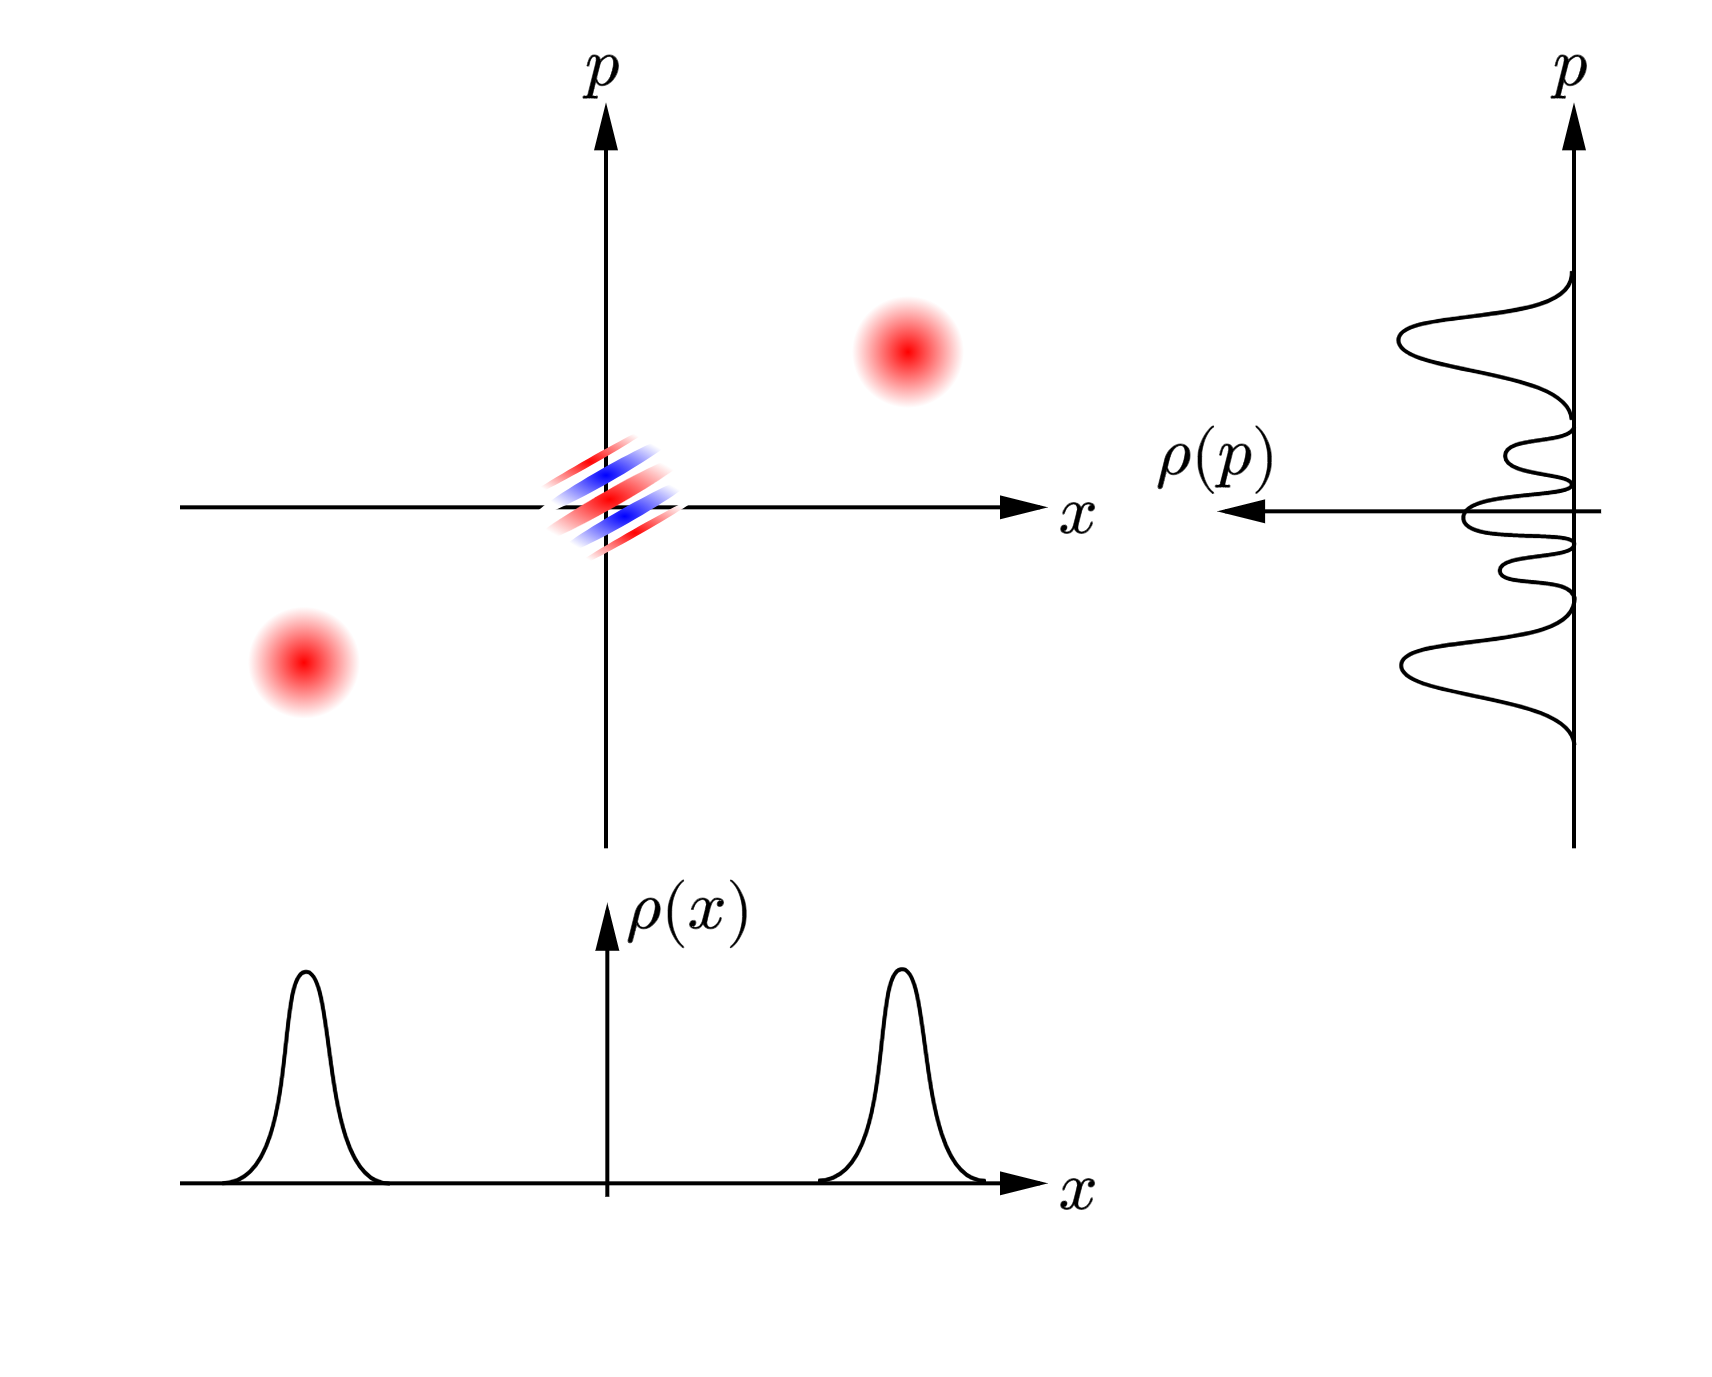
\includegraphics[width=0.6\textwidth]{cat-state.png}
    \caption{The Wigner function of a cat state, and the corresponding $\rho(x)$ and $\rho(p)$.}
    \label{fig:cat-state}
\end{figure}

In a single mode optical field the time evolution is simply to rotate $(\alpha, \alpha^*)$ with angular speed $\omega$.
Therefore, the time evolution of the Wigner function of a cat state is just to rotate \prettyref{fig:cat-state} with angular speed $\omega$.
In this process, the distance between the two peaks on the $x$ axis goes up and down periodically, so the $\rho(x)$ function transforms between a two-peak function and a multiple-peak function where the main peak occurs at $x=0$, the peak value decreasing as $\abs{x}$ increases, and so does $\rho(p)$.
When $\rho(x)$ is a two-peak function $\rho(p)$ is a multiple-peak function, and vice versa.
This is visualized in \cite{cat-state}. 

\paragraph{}

\paragraph{Three-photon state} Consider a three-photon state
\begin{equation}
    \ket*{\psi} = b_1^\dagger b_2^\dagger b_3^\dagger \ket*{0}.
\end{equation}
Calculate the three-photon joint probability $P^{(3)}(\vb*{r}_1, t_2; \vb*{r}_2, t_2; \vb*{r}_3, t_3)$. Analyze the form of the three-photon coherence $g^{(3)}(\vb*{r}_1, \vb*{r}_2, \vb*{r}_3)$ when all the three modes are traveling waves with exactly the same frequency.

\paragraph{Solution} Let $\eta$ be the normalizing constant introduced by constants like $\vb*{d}$ or $\hbar$ in the Fermi's golden rule.
The joint probability is 
\[
    \begin{aligned}
        &\quad P^{(3)}(\vb*{r}_1, t_2; \vb*{r}_2, t_2; \vb*{r}_3, t_3) \\ 
        &= \eta^3 \expval*{E^-(\vb*{r}_1, t_1) E^-(\vb*{r}_2, t_2) E^-(\vb*{r}_3, t_3) E^+(\vb*{r}_3, t_3) E^+(\vb*{r}_2, t_2) E^+(\vb*{r}_1, t_2)} \\
        &= \eta^3 \expval*{b_3 b_2 b_1 E^-(\vb*{r}_1, t_1) E^-(\vb*{r}_2, t_2) E^-(\vb*{r}_3, t_3) E^+(\vb*{r}_3, t_3) E^+(\vb*{r}_2, t_2) E^+(\vb*{r}_1, t_2) b_1^\dagger b_2^\dagger b_3^\dagger}{0}.
    \end{aligned}
\]
By Wick's theorem it can be reduced to the sum of products of two-point correlation functions.
Note that since $E^+ \sim b$, it must contract with a creation operator on its right to create a non-zero two-point correlation function, or in other words all the three $E^+$ operators must contract with $b_1^\dagger, b_2^\dagger, b_3^\dagger$.
So we have 
\[
    \begin{aligned}
        P^{(3)}(\vb*{r}_1, t_2; \vb*{r}_2, t_2; \vb*{r}_3, t_3) &= \eta^3 \times \sum \text{contractions between $b_1, b_2, b_3$ and the three $E^-$s} \\
        &\quad \times \sum \text{contraction between the three $E^+$s and $b_1^\dagger, b_2^\dagger, b_3^\dagger$},
    \end{aligned}
\]
and we immediately notice that again by Wick's theorem 
\[
    \begin{aligned}
        &\quad \sum \text{contraction between the three $E^+$s and $b_1^\dagger, b_2^\dagger, b_3^\dagger$} \\
        &= \mel{0}{E^+(\vb*{r}_3, t_3) E^+(\vb*{r}_2, t_2) E^+(\vb*{r}_1, t_2) b_1^\dagger b_2^\dagger b_3^\dagger}{0} \\
        &= \mel{0}{E^+(\vb*{r}_3, t_3) E^+(\vb*{r}_2, t_2) E^+(\vb*{r}_1, t_2)}{\psi},
    \end{aligned}
\]
and 
\[
    \begin{aligned}
        &\quad \sum \text{contractions between $b_1, b_2, b_3$ and the three $E^-$s} \\
        &= \mel{0}{b_3 b_2 b_1 E^-(\vb*{r}_1, t_1) E^-(\vb*{r}_2, t_2) E^-(\vb*{r}_3, t_3)}{0} \\
        &= \mel{\psi}{E^-(\vb*{r}_1, t_1) E^-(\vb*{r}_2, t_2) E^-(\vb*{r}_3, t_3)}{0},
    \end{aligned}
\]
so 
\begin{equation}
    P^{(3)}(\vb*{r}_1, t_2; \vb*{r}_2, t_2; \vb*{r}_3, t_3) = \eta^3 \abs{\mel{0}{E^+(\vb*{r}_3, t_3) E^+(\vb*{r}_2, t_2) E^+(\vb*{r}_1, t_2)}{\psi}}^2.
    \label{eq:3-photon-probability}
\end{equation}
When $t_1 = t_2 = t_3 = t$, it is just 
\begin{equation}
    P^{(3)}(\vb*{r}_1, \vb*{r}_2, \vb*{r}_3, t) = \eta^3 \abs{\Psi(\vb*{r}_1, \vb*{r}_2, \vb*{r}_3, t)}^2,
\end{equation}
where
\begin{equation}
    \Psi(\vb*{r}_1, \vb*{r}_2, \vb*{r}_3, t) = \mel{0}{E^+(\vb*{r}_3, t) E^+(\vb*{r}_2, t) E^+(\vb*{r}_1, t)}{\psi}
\end{equation}
is the ``three-photon wavefunction''.

Now we evaluate $\mel{0}{E^+(\vb*{r}_3, t_3) E^+(\vb*{r}_2, t_2) E^+(\vb*{r}_1, t_2)}{\psi}$. Again by Wick's theorem
\[
    \begin{aligned}
        &\quad \mel{0}{E^+(\vb*{r}_3, t_3) E^+(\vb*{r}_2, t_2) E^+(\vb*{r}_1, t_2)}{\psi} \\
        &= \sum_{(i, j, k) \in \mathrm{Perm}(\{1, 2, 3\})} \mel{0}{E^+(\vb*{r}_i, t_i) b_1^\dagger}{0} \mel{0}{E^+(\vb*{r}_j, t_j) b_2^\dagger}{0} \mel{0}{E^+(\vb*{r}_k, t_k) b_3^\dagger}{0},
    \end{aligned}
\]
where
\[
    \begin{aligned}
        \expval*{E^+(\vb*{r}_m, t_m) b_n^\dagger}{0} &= \sum_i \mathcal{E}_i f_i(\vb*{r}_m) \expval*{b_i \ee^{- \ii \omega_i t_m } b_n^\dagger}{0} \\
        &= \mathcal{E}_n f_n(\vb*{r}_m) \ee^{-\ii \omega_n t_m}.
    \end{aligned}
\]
Therefore 
\begin{equation}
    \begin{aligned}
        &\quad \mel{0}{E^+(\vb*{r}_3, t_3) E^+(\vb*{r}_2, t_2) E^+(\vb*{r}_1, t_2)}{\psi} \\
        &= \sum_{(i, j, k) \in \mathrm{Perm}(\{1, 2, 3\})} \mathcal{E}_1 \mathcal{E}_2 \mathcal{E}_3 f_1(\vb*{r}_i) f_2(\vb*{r}_j) f_3(\vb*{r}_k) \ee^{- \ii (\omega_1 t_i + \omega_2 t_j + \omega_3 t_k)}.
    \end{aligned}
\end{equation}
Inserting this equation into \eqref{eq:3-photon-probability}, we have obtained an explicit expression of the three-photon joint probability.
Particularly we have 
\begin{equation}
    \Psi(\vb*{r}_1, \vb*{r}_2, \vb*{r}_3, t) = \mathcal{E}_1 \mathcal{E}_2 \mathcal{E}_3 \ee^{- \ii (\omega_1 + \omega_2 + \omega_3) t} \sum_{(i, j, k) \in \mathrm{Perm}(\{1, 2, 3\})}  f_1(\vb*{r}_i) f_2(\vb*{r}_j) f_3(\vb*{r}_k), \quad P^{(3)} = \eta^3 \abs{\Psi}^2.
\end{equation}
It can be observed that $\Psi$ is just symmetrized direct projects of the three ``single photon wave functions'' $f_1, f_2, f_3$.

The definition of three-photon coherence is 
\begin{equation}
    g(\vb*{r}_1, \vb*{r}_2, \vb*{r}_3) = \frac{\expval{E^-(\vb*{r}_1, t) E^-(\vb*{r}_2, t) E^-(\vb*{r}_3, t) E^+(\vb*{r}_3, t) E^+(\vb*{r}_2, t) E^+(\vb*{r}_1, t)}}{\expval{E^-(\vb*{r}_1, t) E^+(\vb*{r}_1, t)} \expval{E^-(\vb*{r}_2, t) E^+(\vb*{r}_2, t)} \expval{E^-(\vb*{r}_3, t) E^+(\vb*{r}_3, t)}}.
\end{equation}
We have already known the numerator. As for the denominator, by Wick's theorem we have
\begin{equation}
    \begin{aligned}
        \expval{E^-(\vb*{r}_1, t) E^+(\vb*{r}_1, t)} &= \mel{0}{b_3 b_2 b_1 E^-(\vb*{r}_1, t) E^+(\vb*{r}_1, t) b_1^\dagger b_2^\dagger b_3^\dagger}{0} \\
        &= \mathcal{E}_1^2 \abs{\vb*{f}_1(\vb*{r}_1)}^2 + \mathcal{E}_2^2 \abs*{\vb*{f}_2(\vb*{r}_1)}^2 + \mathcal{E}_3^2 \abs*{\vb*{f}_3(\vb*{r}_1)}^2.
    \end{aligned}
\end{equation}
Note that if $E^+$ contracts with $b_i^\dagger$ then $E^-$ must contract with $b_i$, or otherwise we will have $\expval*{b_j b_k^\dagger}$ factors where $j \neq k$, which evaluates to zero.

When all the three modes are propagating waves with exactly the same frequency $\omega$, we have
\[
    \vb*{f}_i(\vb*{r}) = \ee^{\ii \vb*{k}_i \cdot \vb*{r}} \vb*{e}_i, \quad i = 1, 2, 3,
\]
and 
\[
    \mathcal{E}_1 = \mathcal{E}_2 = \mathcal{E}_3 = \mathcal{E} = \sqrt{\frac{\hbar \omega}{2 \epsilon_0 V}},
\]
and therefore
\[
    \expval{E^-(\vb*{r}_1, t) E^+(\vb*{r}_1, t)} = 3 \mathcal{E},
\]
and 
\[
    \begin{aligned}
        &\quad \expval{E^-(\vb*{r}_1, t) E^-(\vb*{r}_2, t) E^-(\vb*{r}_3, t) E^+(\vb*{r}_3, t) E^+(\vb*{r}_2, t) E^+(\vb*{r}_1, t)} \\
        &= \abs{\mathcal{E}^3 \sum_{(i, j, k) \in \mathrm{Perm}(\{1, 2, 3\})}  \ee^{\ii (\vb*{k}_1 \cdot \vb*{r}_i + \vb*{k}_2 \cdot \vb*{r}_j + \vb*{k}_3 \cdot \vb*{r}_k )} \vb*{e}_1 \vb*{e}_2 \vb*{e}_3}^2 \\
        &= \mathcal{E}^6 \sum_{\sigma, \sigma' \in \mathrm{Perm}(\{1, 2, 3\})} \prod_{i=1}^3 \ee^{\ii (\vb*{k}_{\sigma(i)} - \vb*{k}_{\sigma'(i)}) \cdot \vb*{r}_i } \vb*{e}_{\sigma(i)} \cdot \vb*{e}_{\sigma'(i)}^*.
    \end{aligned}
\]
Note that permuting $b_1, b_2, b_3$ is equivalent to permuting $\vb*{r}_1, \vb*{r}_2, \vb*{r}_3$, which justifies the third line.
Putting everything together we have
\begin{equation}
    g(\vb*{r}_1, \vb*{r}_2, \vb*{r}_3) = \sum_{\sigma, \sigma' \in \mathrm{Perm}(\{1, 2, 3\})} \prod_{i=1}^3 \ee^{\ii (\vb*{k}_{\sigma(i)} - \vb*{k}_{\sigma'(i)}) \cdot \vb*{r}_i } \vb*{e}_{\sigma(i)} \cdot \vb*{e}_{\sigma'(i)}^*.
\end{equation}

\bibliographystyle{plain}
\bibliography{../optics/quantize,1} 

\end{document}